\documentclass[a4paper, 12pt]{article}
\usepackage{cmap}
\usepackage[warn]{mathtext}
\usepackage[T2A]{fontenc}
\usepackage[utf8]{inputenc}
\usepackage{graphicx}
\usepackage{amssymb}
\usepackage{amsmath}
\usepackage{wrapfig}
\usepackage{siunitx}
\graphicspath{image/}
\title{Исследование прецессии уравновешенного гироскопа}
\author{Шакиров Тимур Тагирович}
\date{Ноябрь 2021}
\renewcommand{\figurename}{Рис.}
\begin{document}

\maketitle

\textbf{Цель работы:} исследовать вынужденную прецессию гироскопа; установить зависимость скорости вынужденной прецессии от величины момента сил, действующих на ось гироскопа; определить скорость вращения ротора гироскопа и сравнить ее со скоростью, рассчитанной по скорости прецессии.

\vspace{1cm}

\textbf{В работе используются:} гироскоп в кардановом подвесе, секундомер, набор грузов, отдельный ротор гироскопа, цилиндр известной массы, крутильный маятник, штангенциркуль, линейка, осцилограф.

\vspace{1cm}

\section*{Теория}
Момент импульса тела в его осях $x$, $y$, $z$:
\begin{equation}
    \label{e1}
    \bar{L}=\bar{i}I_x\omega_x+\bar{j}I_y\omega_y+\bar{k}I_z\omega_z.
\end{equation}
Гироскоп---быстро вращающееся тело, для которого 
\begin{equation}
    \label{e2}
    I_z\omega_z\gg I_x\omega_x,\hspace{0.25cm} I_y\omega_y.
\end{equation}
Гироскоп называют уравновешенным, если его центр масс неподвижен.
Приращение момента импульса определяется интегралом
\begin{equation}
    \label{e3}
    \Delta \bar{L}=\int \bar{M} dt
\end{equation}
Для малого промежутка времени $|\Delta\bar{L}|\ll |\bar{L}|$
Рассмотрим, какие силы нужно приложить к гироскопу, чтобы изменить положение его оси вращения:
\begin{wrapfigure}[20]{l}{180pt}
    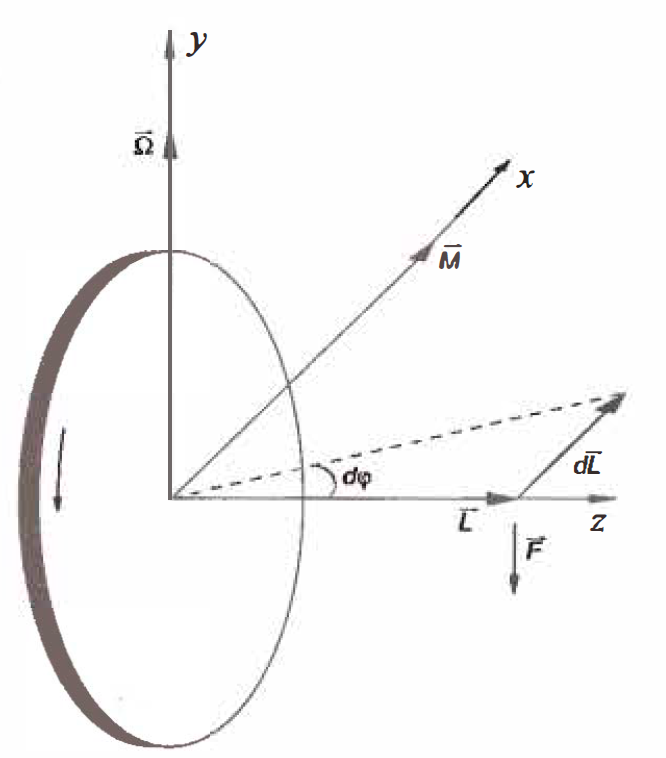
\includegraphics[width=180pt]{image/png1.png}
    \caption{\label{p1}Маховик}
\end{wrapfigure}
$d\varphi=\Omega dt \hspace{1cm} L_\Omega \ll L$\\
$|d\bar{L}|=Ld\varphi=L\Omega dt$\\
$d\bar{L}=\bar{\Omega}\times\bar{L}dt$\\
\begin{equation}
    \label{e4}
    \bar{M}=\bar{\Omega}\times\bar{L}
\end{equation}

Под действием $\bar{M}$ ось гироскопа медленно вращается вокруг $OY$ с $\Omega$. Такое движение называется регулярной прецессией гироскопа.
Для гироскопа, у которого ось вращения отклонена на угол $\alpha$ от вертикали:
\begin{equation}
    \Omega=\frac{mgr}{I\omega}
    \label{e5}
\end{equation}
Момент инерции $I$ гироскопа можно найти с помощью крутильных колебаний.
$T_0=2\pi\sqrt{\frac{I}{f}}$, $T_1=2\pi\sqrt{\frac{I_1}{f}}$, значит
\begin{equation}
    \label{e6}
    I=I_1\frac{T_0^2}{T_1^2},
\end{equation}
где $f$---модуль кручения проволоки, $I_1$---известный момент инерции цилиндра, а $T_0$ и $T_1$---периоды колебаний гироскопа и цилиндра соответственно.\\
Скорость вращения ротора можно измерить и с помощью осциллографа. Ротор, вращаясь, наводит ЭДС в обмотке, но при включенном в сеть гироскопе наводит ЭДС не только он, но и раскручивающая ротор обмотка. Так что для корректного измерения частоты вращения ротора гироскоп нужно выключать из сети.
\section*{Ход работы}
\begin{enumerate}
    \item Установили ось гироскопа в горизонтальное положение.
    \item Включили питание гироскопа и подождали стабилизации вращения ротора.
    \item Убедились в устойчивости гироскопа. С помощью уравнения (\ref{e4}) определили сторону вращения ротора, приложив момент сил к гироскопу.
    \item
    Подвесили к рычагу груз. Пронаблюдали прецессию. В ходе прецессии рычаг медленно опускался. К этому приводит трение в вертикальной оси. Суммарный момент сил трения вертикальной оси $\bar{M_{fr}}$ направлен вниз, а значит и $d\bar{L}$ тоже.
    \begin{figure}[h]
    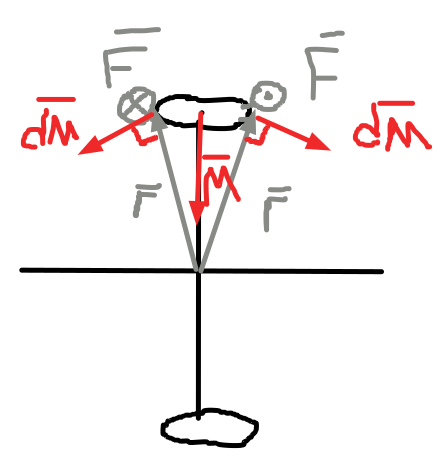
\includegraphics[width=120pt]{image/mfr.png}
    \end{figure}
    \item Отклонили конец рычага на $x=10\text{мм}$, то есть на угол $\alpha=\frac{x}{l}\frac{2\pi}{360}\approx 5 $ градусов, где $l$---расстояние от вертикальной оси до конца рычага. Наблюдали прецессию до тех пор, пока рычаг не опустится на 5 градусов ниже горизонтальной плоскости. По количеству оборотов, углу $\alpha$ и времени прецессии нашли $\Omega$, $\Omega_{fr}$, где $\Omega_{fr}$---скорость опускания рычага. Результаты внесли в таблицу.
    \begin{table}[h]
    \centering
    \begin{tabular}{|l|lll|}
    \hline
    t, c & n & T, c & $\Omega$ , $c^{-1}$ \\ \hline
    136 & 4.5 & 30.2 & 0.21 \\ 
    136 & 4.5 & 30.2 & 0.21 \\ 
    152 & 5 & 30.4 & 0.21 \\ 
    152 & 5 & 30.4 & 0.21 \\ 
    151 & 5 & 30.4 & 0.21 \\ \hline
    \end{tabular}
    \end{table}\\
    \begin{equation*}
        \overline{\Omega}_1=\frac{\sum_{i=1}^5 \Omega_i}{5}=0.21
    \end{equation*}
    \item Провели серию экспериментов, описанных в п.5, с другими $\bar{M}$, результаты внесли в таблицу.\\
    \begin{table}[h]
    \centering
    \begin{tabular}{|l|rrrrrrr|}
    \hline
    {} &         1 &         2 &         3 &         4 &         5 &         6 &         7 \\ \hline
    $M, H\cdot m$   &  0.40 &  0.32 &  0.25 &  0.20 &  0.16 &  0.13 &  0.10 \\ 
    $\Omega,c^{-1}$ &  0.20 &  0.16 &  0.13 &  0.10 &  0.08 &  0.06 &  0.05 \\ \hline
    \end{tabular}
    \end{table} \\
    График $\Omega$ от $M$ представлен в конце отчета.
    \item Измерили момент инерции ротора гироскопа относительно оси симметрии $I_0$. Зная периоды крутильных колебаний $T_0$ и $T_1$ ротора и цилиндра с известным $I_1$ соответственно нашли $I_0$ по формуле (\ref{e6}).\\
    \begin{table}[h]
    \centering
    \begin{tabular}{|l|rrrr|}
    \hline
    {} &      1 &      2 &      3 &    $T_{ср}$ \\ \hline
    $T_0$ &  3.13 &  3.15 &  3.19 &  3.16 \\
    $T_1$ &  4.08 &  4.00 &  4.03 &  4.03 \\
    \hline
    \end{tabular}
    \end{table}\\
    $I_1=m_c\frac{D^2}{8}=0.0012$ кг$\cdotм^2$\\
    $I_0=I_1\frac{T_0^2}{T_1^2}=0.0008$ кг$\cdotм^2$
    \item Оценка погрешностей произведена в п.12.
    \item С помощью (\ref{e5}) рассчитаем $\omega$.\\
    $\omega=\frac{M}{I_0\Omega}$\\
    \begin{table}[h]
        \centering
        \begin{tabular}{|l|rrrrrrr|}
        \hline
        {} &           1 &           2 &           3 &           4 &          5 &           6 &           7 \\ \hline
        $M, H\cdot m$   &    0.40 &    0.32 &    0.26 &    0.21 &    0.17 &    0.14 &    0.11 \\ 
        $\omega,c^{-1}$ &  2500& 2630& 2630& 2510& 2480& 2630& 2410 \\
        \hline
\end{tabular}

    \end{table}\\
    $\omega_{ср}=2540 c^{-1}$
    \item Определим момент сил трения в оси. \\
    $M_{fr}=\frac{2L\alpha}{t}=\frac{2\alpha I\omega}{t}$
    \begin{table}[h]
        \centering
    \begin{tabular}{|l|rrrrrrr|}
    \hline
    {} &    1 &    2 &    3 &    4 &    5 &    6 &    7\\
    \hline
    $t,c$ &  151 &  154 &  143 &  144 &  145 &  180 &  166 \\
    $\Omega_{fr}, c^{-1}$& 0.042&  0.041&  0.044& 0.044& 0.043& 0.034&   0.038 \\
    $M_{fr}, H\cdot m$& 0.083& 0.085& 0.092& 0.087& 0.086& 0.073& 0.073 \\
    \hline
    \end{tabular}
    \end{table} \\
    $M_{fr}=0.083$ H$\cdot $m
    \item С помощью осциллографа и генератора измерим частоту вращения ротора. Изменяя частоту генератора добьемся появления неподвижного эллипса. При этом питание ротора должно быть выключено.\\
    $\nu=390$ Гц, $\omega=2450c^{-1}$
    \item Оценим погрешности полученных величин.
    $\varepsilon_D\approx 0.001$\\
    $\varepsilon_{m_c}\approx 0.0001$\\
    $\varepsilon_{I_1}=\sqrt{4\varepsilon_D^2+\varepsilon_{m_c}^2}=0.001$\\
    $\sigma^{\text{сл}}_T = \sqrt{\frac{1}{N - 1} \sum_{i = 1}^{N} \left(T_i -  T_{ср} \right)^2}=0.02c$\\
    $\sigma^{\text{сист}}_T=0.02c$\\
    $\sigma_T=0.03c$\\
    $\varepsilon_{I_0}=\sqrt{\varepsilon_{I_1}^2+8\varepsilon_{T}^2}=0.03$\\
    $\varepsilon_{\Omega}=\varepsilon_T=0.01$ \\
    $\varepsilon_{\alpha}\approx\varepsilon_{2x}=0.05$\\
    $\sigma^{\text{сл}}_{\omega} = \sqrt{\frac{1}{N - 1} \sum_{i = 1}^{N} \left(\omega_i -  \omega_{ср} \right)^2}=80c^{-1}$\\
    $\sigma^{\text{сист}}_{\omega}=\omega \varepsilon_{\omega}^{сист}\approx\omega\varepsilon_{I_0}=70c^{-1}$\\
    $\sigma_{\omega}=90c^{-1}$\\
    $\varepsilon_{M_{fr}}=\sqrt{\varepsilon_{\alpha}^2+\varepsilon_I^2+\varepsilon_{\omega}^2+\varepsilon_t^2}\approx 0.06$\\
    $\omega=(2540\pm 90)c^{-1}$\\
    Значение угловой скорости вращения ротора гироскопа, полученное с помощью прецессии, совпадает со значением, полученным с помощью осциллографа в пределах погрешности.
    
    
\end{enumerate}
\newpage
\section*{Приложение}
    \begin{figure}[h]
        \centering
        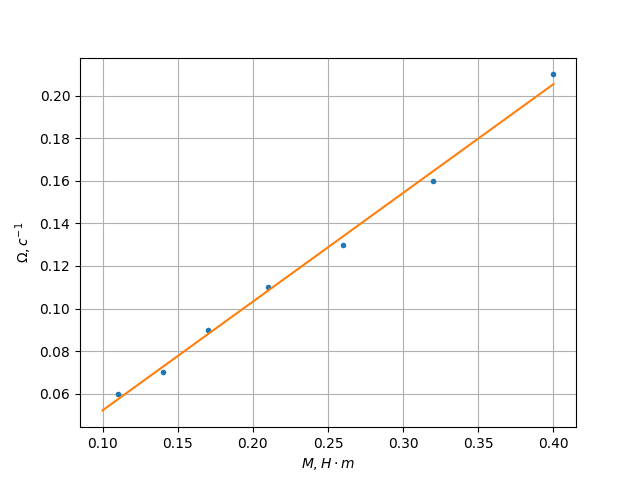
\includegraphics{image/Figure_1.png}
    \end{figure}

\end{document}
